\documentclass[english,hidelinks]{sbrt}
\usepackage{newtxtext}
\usepackage[english]{babel}
\usepackage[utf8]{inputenc}
\usepackage{xurl,graphicx,flushend,hyperref}
\setlength{\textfloatsep}{8pt plus 2pt minus 2pt}
\setlength{\intextsep}{8pt plus 2pt minus 2pt}
\raggedbottom
\begin{document}
\nocite{IEEEcontrol}
\title{A Panic Button for Everyday Carry with Smartphone-Independent Location Fallback}
\author{Letícia Valladão and Vinicius Dias\thanks{Computer Engineering, Ibmec, Brazil.}}
\maketitle
\markboth{IBMEC -- IBM3118 EMBEDDED SYSTEMS -- AP2, 2026.2}{}
\begin{abstract}
A wearable panic button must remain available through long periods of inactivity and still initiate an alert when the user's phone is out of reach. We implemented two activation methods on an ESP32 and a controller that first requests a location over Bluetooth Low Energy (BLE), then turns to a GNSS receiver if the request expires. A USB bench emulator supplied GNSS sentences and cellular modem responses. The ESP32 recognized a Portuguese keyword in 48 of 50 attempts in quiet and 48 of 50 with background video. Under the same 2{,}000 mAh battery model, estimated standby lifetime fell from 12{,}500 h with a physical wake button to 43 h with continuous listening at 160 MHz.
\end{abstract}
\begin{keywords}
Wearable emergency device, Bluetooth Low Energy, deep sleep, keyword spotting, GNSS.
\end{keywords}
\section{Introduction}
For a person seeking help, the first obstacle may be reaching the phone used to raise the alarm. A systematic review of mobile applications addressing violence against women found a prevalence of emergency interventions and little evidence of their effectiveness \cite{eisenhut}. A mapping study of wearables for the prevention of sexual violence documents a second design option: moving the trigger onto an object the user can carry or wear \cite{paiva}. A wearable trigger, however, can still depend on the phone for its position.

A device carried daily may spend most of its service life waiting for an event. Measurements of embedded communication systems show how strongly radio duty cycle influences battery life \cite{caracas2011energy}. Measurements on the ESP32 likewise show that the choice of sleep state changes the average current drawn by a monitoring application \cite{dzahir2023evaluating}. For a panic button, the relevant question is how much energy each activation method consumes while the user is doing nothing.

Existing devices illustrate the choices. SMARISA uses a ring to initiate an alert and obtains position through the user's phone \cite{sogi2018smarisa}. Mallapur et al. integrate GPS and GSM on the device and report 8--10 h of standby \cite{mallapur2025emergency}. SafeGuard Bangle incorporates a physical emergency trigger \cite{mishra2025safeguard}. Purnima et al. combine positioning, cellular messaging and image capture \cite{purnima2025wearable}. Sudheer et al. evaluate a safety device across connectivity conditions \cite{sudheer2025emergency}. GNSS reception indoors remains sensitive to attenuation and obstruction \cite{dedes2005indoor}.

We implement phone-assisted positioning with a GNSS fallback and evaluate physical and spoken activation on the same ESP32. Bench tests characterize reconnection, keyword detection and recovery from loss of the phone. A component-level model estimates battery life in standby and during reporting. The project repository accompanies this study \cite{repo}.

Sections II and III describe the prototype and its control logic. Section IV evaluates timing, detection and energy. Section V discusses everyday use and hardware integration.

\section{System and problem formulation}
The intended device comprises an ESP32, a push button, a GNSS receiver (NEO-6M), a GSM modem (SIM800L) and a battery. The ESP32 provides BLE and deep sleep \cite{dzahir2023evaluating}. The receiver and modem implement the GPS/GSM architecture also used in wearable alerts \cite{mallapur2025emergency,purnima2025wearable}. The phone supplies coordinates when available. The modem is the intended message transport on both paths. Losing the Bluetooth link must therefore change how the device obtains its position while preserving the emergency state. Figure~\ref{fig:flow} shows the first report from activation to the message request.

\begin{figure}[!htbp]
\centering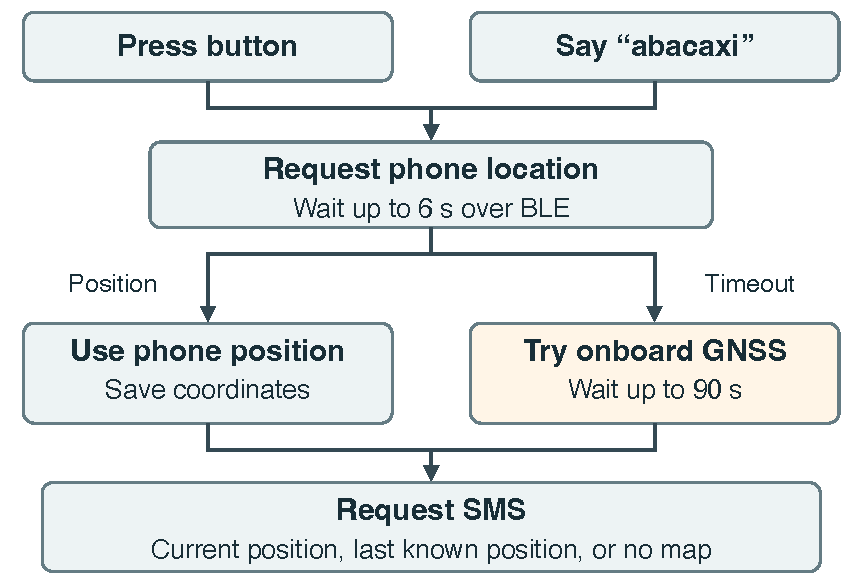
\includegraphics[width=\columnwidth]{flow.pdf}
\caption{First report after activation. After a phone timeout, subsequent reports use GNSS directly until cancellation.}
\label{fig:flow}
\end{figure}
The bench prototype uses an ESP32-WROVER development board. A Mac supplies microphone samples and emulates the two unavailable peripherals over USB. The firmware reads NMEA position sentences and issues SMS commands to the modem interface. The emulator can forward the resulting text to Telegram. A modem acceptance event and a Telegram delivery event are logged separately. The physical GNSS receiver, cellular network, battery and final enclosure remain outside the evaluated prototype.

\section{Activation and reporting methods}
In button-only mode the ESP32 remains in deep sleep until the push button wakes it. In voice-enabled mode it stays awake at 160 MHz and accepts either the button or the keyword ``abacaxi''. Mono audio sampled at 16 kHz is processed on the ESP32 in 250 ms slices of a one-second window. A detection requires two consecutive keyword scores of at least 0.80. Both triggers call the same emergency routine. This isolates the energy cost of listening from the later cost of locating and sending.

The ESP32 must extract features and classify each slice before the next 250 ms of audio arrive. Replacing the transfer-learning classifier reduced estimated inference time from 826 to 11 ms and classifier RAM from 166.2 to 14.7 kB. These estimates exclude audio capture and feature extraction.

At the first report (Fig.~\ref{fig:flow}), the ESP32 advertises its BLE service. A connected client receives an alert request and writes latitude, longitude and estimated accuracy. If a valid position arrives within the deadline T, the device uses it. Otherwise it requests GNSS, waits up to 90 s for a valid fix and switches subsequent reports in that emergency directly to GNSS. If no fix arrives, the controller uses the last known position when available. Firmware for the demonstration sends an alert without a map when no position has ever been obtained.

On the bench, the Mac supplies position sentences over USB. The ESP32 verifies each RMC sentence against its checksum, checks that the receiver marks the fix as valid, and converts latitude and longitude from degrees and minutes to signed decimal degrees. A malformed sentence leaves the acquisition routine waiting for another fix. If the acquisition window closes first, the firmware identifies any stored coordinates as the last known position in the alert. This distinction lets a recipient interpret the map point even when a fresh fix is unavailable.

RTC memory preserves the emergency flag, report counter, next deadline and last known coordinates across sleep. Scheduling each report from activation prevents acquisition and transmission delays from accumulating when they fit within the reporting interval (60 s on the bench). Holding the button for 3 s cancels the emergency, even during a GNSS wait. The prototype includes a native macOS BLE client. Timing trials used the AP1 browser client on the Mac.

\section{Results and discussion}
\emph{Bluetooth timing.} In the browser experiment the awake board obtained 16 acknowledgements in 16 trials (median 0.555 s). After deep sleep, 21 of 22 trials obtained a phone-path acknowledgement. Two required manual reconnection after a browser prompt and one took the fallback path. Among the 19 automatic successes, the median time from firmware startup to acknowledgement was 2.602 s (range 2.039--5.262 s). ROM boot time is excluded. The browser usually reused a cached location. The notebook obtained its position over Wi-Fi and reported an estimated accuracy of about 35 m. This was the location provider's own uncertainty estimate. The experiment had no surveyed reference point against which to measure positioning error. The AP1 browser awaited its Telegram request before writing coordinates back. Timing ended when the ESP32 received that acknowledgement. The current client writes the acknowledgement first.

\begin{figure}[!htbp]
\centering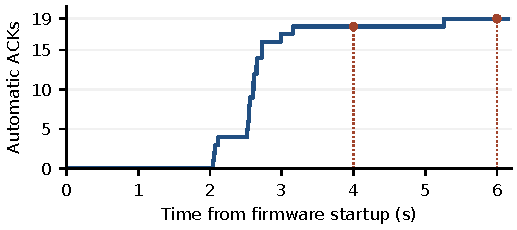
\includegraphics[width=\columnwidth]{deadline.pdf}
\caption{Cumulative automatic BLE acknowledgements after wake-up ($n=19$, observation window 60 s).}
\label{fig:deadline}
\end{figure}
\emph{Deadline choice.} Within the 60 s observation window, 18 of 19 automatic acknowledgements arrived by 4 s and all 19 by 5.262 s (Fig.~\ref{fig:deadline}). The slowest included a 2.631 s fresh location request, whereas median BLE reconnection took only 0.615 s. We therefore select 6 s, allowing 0.738 s beyond the observed maximum and starting fallback 9 s earlier than the original 15 s setting when the phone is absent. New trials must validate this retrospective choice. The two manual reconnections also show why the controller needs a fallback when the browser waits for user input.

\emph{Voice activation.} The ESP32 recognized 96\% of intentional utterances in each acoustic condition. In quiet, the median interval from the estimated end of speech to the host receiving the detection was 216 ms (48 detections). Latency is reported for quiet trials only.

Table~\ref{tab:voice} reports the four runs separately. Although both conditions yielded 48 detections in 50 attempts, the misses were distributed differently across runs. The background-video condition also exposed a limitation of the timing instrument: the host could receive the keyword event even when its speech detector could not reliably identify when the speaker stopped talking. A separate observation period without intentional keywords is needed to estimate false activations.

\begin{table}[!htbp]
\centering
\caption{Intentional keyword trials on the ESP32, in recording order.}
\label{tab:voice}
\begin{tabular*}{\columnwidth}{@{\extracolsep{\fill}}clrr@{}}
\hline
Run & Acoustic condition & Detected & Missed \\
\hline
1 & Quiet & 28/30 & 2 \\
2 & Background video & 19/20 & 1 \\
3 & Background video & 29/30 & 1 \\
4 & Quiet & 20/20 & 0 \\
\hline
\end{tabular*}
\end{table}

\begin{figure}[!htbp]
\centering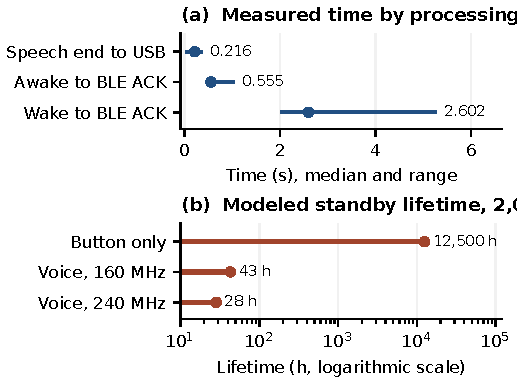
\includegraphics[width=\columnwidth]{profiles.pdf}
\caption{(a) Median and range for voice detection in quiet ($n=48$) and BLE acknowledgement while awake ($n=16$) or after wake-up ($n=19$). (b) Modeled standby lifetime.}
\label{fig:profiles}
\end{figure}
Figure~\ref{fig:profiles} distinguishes two stages. Voice timing ends at the USB detection record. BLE timing ends when the board receives the browser acknowledgement. Waking from sleep added 2.047 s between BLE medians. Ranking the triggers by response time would require a common endpoint, such as entry into the emergency routine.

\emph{Energy model.} Standby lifetime is battery capacity divided by average current. Using device datasheets and the assumptions listed in the simulation \cite{repo}, button standby draws 0.010 mA for the sleeping ESP32 plus 0.150 mA for modem power-down. Listening at 160 MHz adds the modeled 44 mA processor and 2.5 mA microphone loads in place of the sleeping processor. At 240 MHz the processor assumption is 68 mA. Reducing the listening clock raises estimated standby lifetime from 28 to 43 h. The estimates exclude board-level losses and self-discharge. They apply to a proposed battery-powered assembly, not to the USB-powered board.

For recurring reports, the model weights current by time in each phase and uses the AP1 median ACK time as a proxy for the phone stage. At a four-minute reporting interval, it projects 325 h using phone coordinates and 113 h using repeated cold GNSS fixes (Fig.~\ref{fig:energy_lifetime}). Longer intervals amortize acquisition energy at the cost of less frequent updates. The model assumes 27 s per cold fix, 3 s per SMS, a registered modem between reports and a transmit-current proxy for SMS. Steady-state estimates exclude the first phone timeout. With one-minute updates, the projections fall to 93 h with phone coordinates and 30 h with cold GNSS acquisition. Moving to four minutes extends the projected operating time on either path, but a contact then has to wait three minutes longer between scheduled updates.

\begin{figure}[!htbp]
\centering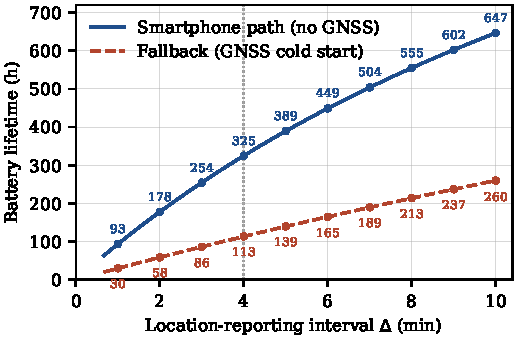
\includegraphics[width=\columnwidth]{energy_lifetime.pdf}
\caption{Modeled battery life versus reporting interval. The vertical line marks four minutes between location updates.}
\label{fig:energy_lifetime}
\end{figure}

Bench traces also exercised failures that a latency median cannot capture. In one sequence the client supplied the first position and became unavailable before a later report. The controller switched to the emulated receiver and bypassed BLE on subsequent reports in that emergency. In a separate timeout case it issued a message using the last known position. The location in such a message describes an earlier observation. These trials verify the controller logic under loss of an input. Radio coverage and the age and accuracy of real fixes require field testing.

\section{Conclusions}
For an everyday device carried for long periods between emergencies, the results favor waking the ESP32 with a physical button. The controller retained emergency state across reports and recovered from loss of the phone on the bench. In the AP1 browser trials, the median time to acknowledgement increased by about two seconds after deep sleep. Continuous listening offers hands-free activation, but its modeled standby current at 160 MHz is about 292 times that of the button profile. For someone who can reach the button, deep sleep makes it practical to carry the device through long periods of inactivity with little attention to charging. Voice becomes especially valuable when the hands are occupied or the trigger is out of reach. A pocket-sized version could accommodate a larger rechargeable battery, but microphone placement and recognition through clothing would then become design requirements.

The next step is to integrate the receiver, modem, microphone and battery in a wearable enclosure, measure standby current and verify end-to-end SMS delivery with the phone unavailable. Current should be measured over complete wake, acquisition and transmit cycles as well as in standby. Comparing those measurements with the model would show whether the dominant cost is the listening processor, GNSS acquisition or cellular transmission in the assembled device. Field trials can then assess indoor and outdoor positioning and the false-activation rate during everyday use.

\bibliographystyle{IEEEtran}
\bibliography{refs}
\end{document}
